\documentclass[conference]{IEEEtran}
\usepackage{times}

% numbers option provides compact numerical references in the text. 
\usepackage[numbers]{natbib}
\usepackage{multicol}
\usepackage[bookmarks=true]{hyperref}
\usepackage{graphicx,mathrsfs}


\pdfinfo{
   /Author (Homer Simpson)
   /Title  (Robots: Our new overlords)
   /CreationDate (D:20101201120000)
   /Subject (Robots)
   /Keywords (Robots;Overlords)
}

\begin{document}

% paper title
\title{Learning Simultaneous Sensory and Motor Representations- (SESEMO)}

% You will get a Paper-ID when submitting a pdf file to the conference system
\author{Berkeley Kids}

%\author{\authorblockN{Michael Shell}
%\authorblockA{School of Electrical and\\Computer Engineering\\
%Georgia Institute of Technology\\
%Atlanta, Georgia 30332--0250\\
%Email: mshell@ece.gatech.edu}
%\and
%\authorblockN{Homer Simpson}
%\authorblockA{Twentieth Century Fox\\
%Springfield, USA\\
%Email: homer@thesimpsons.com}
%\and
%\authorblockN{James Kirk\\ and Montgomery Scott}
%\authorblockA{Starfleet Academy\\
%San Francisco, California 96678-2391\\
%Telephone: (800) 555--1212\\
%Fax: (888) 555--1212}}


% avoiding spaces at the end of the author lines is not a problem with
% conference papers because we don't use \thanks or \IEEEmembership


% for over three affiliations, or if they all won't fit within the width
% of the page, use this alternative format:
% 
%\author{\authorblockN{Michael Shell\authorrefmark{1},
%Homer Simpson\authorrefmark{2},
%James Kirk\authorrefmark{3}, 
%Montgomery Scott\authorrefmark{3} and
%Eldon Tyrell\authorrefmark{4}}
%\authorblockA{\authorrefmark{1}School of Electrical and Computer Engineering\\
%Georgia Institute of Technology,
%Atlanta, Georgia 30332--0250\\ Email: mshell@ece.gatech.edu}
%\authorblockA{\authorrefmark{2}Twentieth Century Fox, Springfield, USA\\
%Email: homer@thesimpsons.com}
%\authorblockA{\authorrefmark{3}Starfleet Academy, San Francisco, California 96678-2391\\
%Telephone: (800) 555--1212, Fax: (888) 555--1212}
%\authorblockA{\authorrefmark{4}Tyrell Inc., 123 Replicant Street, Los Angeles, California 90210--4321}}


\maketitle

\begin{abstract}
\end{abstract}

\IEEEpeerreviewmaketitle




Redundancy reduction \cite{barlow1961possible}, edge detection \cite{hubel1968receptive}  and hierarchical representations \cite{krizhevsky2012imagenet} have been the main stay for lot of work in computer vision and vision neuroscience to represent sensory data. But, these representations do not directly lend themselves to action. It has been argued elsewhere \cite{o2001sensorimotor} that what the brain probably codes for are an organism's sensorimotor contingencies.  

Work by Philipona and O'Regan \cite{philipona2003there,philipona2003perception} showed that the dimensionality of the manifold of compensable actions is smaller than the dimensionality of the sensory or motor spaces. How then can we go about building a model that models the manifold of the sensory space but with knowledge of it's relationship with the motor system? 

In this work we wish to explore this problem by introducing two ideas 
\begin{itemize}
\item Learning a basis space that represent motor actions 
\item Joint estimation of both sensory and motor representations
\end{itemize}


\section{Model}
\textbf{I} is the Image that falls on the retina (say). From this image, we learn our sensory representation \textbf{S}. From \textbf{S}, we infer our representation \textbf{$\alpha$}. We then apply a matrix transformation $\mathcal{G}$ that takes us from the sensory space to the motor actuator space. Here, we learn a motor representation \textbf{M} and the coefficients \textbf{$\beta$} are not inferred but are a transformation based on the sensory estimate. The transformation $\mathcal{F}$ tries to describe the complex non-linear coupling that links motor actions to changes in sensory states. This is complex and nonlinear because the same action performed at different times depending on the sensory state of the world can have completely different outcomes, here in lies the challenge of working with this problem

\begin{figure}
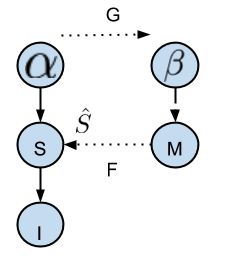
\includegraphics[scale=0.6]{sesemo1.png}
\caption{A loosely defined graphical model that describes the problem sensorimotor representations. }
\end{figure}

In our case, we define the objective to be tracking a point light source in a virtual world. We are given a camera plane and two motors that control the camera. Further, we parameterize the motor space. That is, to move the camera in the x-y plane all we have to do is apply varying powers to the two different motors. In stead of solving for the appropriate amount of power at each time step, we put forward an idea of motor representation for controlling the camera. This motor representation is a collection of tuples that specify the power to the two different motors. 

\begin{eqnarray}
\min_{S,\alpha^{t}} \| I - S\alpha^{t} \|_{2} + \lambda \| \alpha^{t} \|_{1}\\
\min_{G,M}  \| dx - (center + \beta_{t+1}^{T}M ) \|_{2} + \|G \|_{2}\\
\textit{where}\\
\beta_{t+1} = \alpha_{t} G
\end{eqnarray}

The way we go about solving the various parameters is by solving the problem in stages. The interesting idea with this model is that the sensory representation can be learnt independently as well with little loss of generality. For the rest of this work, we will not describe talking about learning the Sensory representations and focus on trying to learn the Motor basis with coefficients that are not inferred but are transformed (G) versions of inferred sensory coefficients. For our experiments we also fix our Sensory basis (S) to be a bunch of vectors that point in eight different directions that the light source may have traveled from the previous frame.

An important point to note is that our model is not completely without supervision. For the model to learn the consequences of it's motor actions we use a teacher signal (dx) that tells the system how the motor actions effect the state of the system. Another point of interest is that we begin our system with the agent not knowing the dynamics of it's control system. That is, it does not know what forward/backward/left/right are but by minimizing a global objective function it learns how to control it's motor to attain specific trajectories. 

The data in this case are 10000 samples of a point light source moving according to the following equation 
\begin{eqnarray}
r = a + b cos(k \theta),\textit{where } \theta = [ -\pi, \pi ] \\
x = r cos(\theta)\\
y = r sin(\theta)\\
\end{eqnarray}

To solve (equation 2.2) we take our current estimate of $\alpha$ and multiply it with matrix $G$ (which is either learnt or fixed as a random matrix). This is our estimate of $\beta$. We then solve for M,G using BFGS as the solver. The model learns pretty quickly and takes only a few 100 samples to converge. We then test our model on a different value of k in the above equation for about 100 samples.

The results of our experiments are summarized in the table below. Row 1 describes the experiments with learning only the Motor basis. Row 2 describes experiments with learning both the motor basis M and the sensorimotor transform G. Row 3 describes experiments with learning both the Motor basis (M) and the sensorimotor transform G but with an extra constraint on minimizing the norm of G. From our experiments, this was the best model. Systemic errors occurred during the sharp turns that we see in the data, we hypothesize that with a more sophisticated planning component in the motor planning part of the model, this can be overcome. The motor space learnt tiles the set of directions we would want the camera to move in, increasing the over completeness resulted in a more granular representation of the 3D space.

\begin{figure}
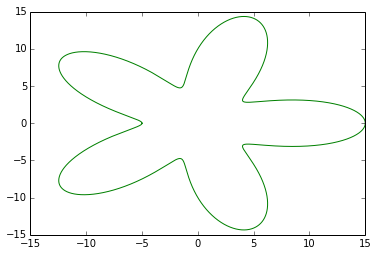
\includegraphics[scale=0.6]{train1.png}
\caption{A loosely defined graphical model that describes the problem sensorimotor representations. }
\end{figure}

% Requires the booktabs if the memoir class is not being used
\begin{table}[htbp]
   \centering
   %\topcaption{Table captions are better up top} % requires the topcapt package
   \begin{tabular}{@{} lcr @{}} % Column formatting, @{} suppresses leading/trailing space
      \multicolumn{2}{c}{A Comparison of Models } \\
      \textbf{Model}    & \textbf{Error} (\$)\\
      \hline
      M      & 68.01 \\                
      M,G       &  13.95 \\
      M,$\|G\|_{2}$       & 0.58 \\
      
   \end{tabular}
   \caption{The table depicts the errors we see while learning variations of the model.}
   \label{tab:booktabs}
\end{table}

\section{Discussion}

We present preliminary work in trying to explore a model that tries to learn a motor representation to track an object based on its sensory representations. We show that a simple model can be learnt without having to learn the effects of the motor actions on the sensory space directly, which is a high dimensional, non-linear and complex space. We argue that by posing problems in this way with a global objective, we can explore various parts of the control space effectively because it is bounded by the task and the sensory representation. Similarly, the sensory representation that is learnt (not done in this work) is also directed towards action as opposed to a representation that is purely for redundancy reduction (compression) or to ask questions such as object recognition.

Future work, can look towards extending this model to more complicated examples such as tracking real world objects with clutter and background noise. Longer term temporal dependencies in both sensory and motor representations can and should be learnt. Exploring complex planning strategies on a motor representation by combinatorically arranging motor basis is also a direction that needs to be explored that biology has learnt to solve in higher mammals such as macaques, dolphins and humans.

\section{ Acknowledgments} 

This work was done in close collaboration with Pulkit Agarwal, EECS, Berkeley. Discussions with Jitendra Malik and Tony Bell motivated a lot of this work as well. Special thanks to Pavan Ramkumar, Northwestern University for helping clarify a lot of ideas through discussions. Special thanks to Bruno Olshausen for urging us to think about sensorimotor representations. 

All the code for this project can be found on our github\footnote{github.com/rctn/sesemo} link.

\section{Acknowledgments}
Ack - Bruno Olshausen. Funding agencies. 


\bibliography{cs287_final}
\bibliographystyle{plainnat}

\end{document}


